% Provenance (never printed): see sources/outline_sources.md (Year 1: hotspots and
% mantle plumes; hotspot chains and absolute plate motion; large igneous provinces).
% Hotspot map, pole fit, rates and swell from figdata/bachelor-1/hotspots.py (data
% data/derived/bachelor-1-hotspots.csv, Table 1 of the Morgan and Morgan 2007 electronic
% supplement); exercise and problem values in the Book 3 scratch calculators calc/ch15.py and
% calc/ch15ex.py. "Hotspot" is re-founded from Book 1 (g7 volcanoes), "hotspot track"
% from Book 2 (g11 plate-motions); Book 2 owns the age--distance fit of the Hawaiian
% chain, so this chapter fits the Pacific Euler pole from track directions instead.
\chapter{Hotspots en intraplaatvulkanisme}\label{ch:b1:hotspots}

Vanaf januari 1983, en tientallen jaren daarna, barstte de Kilauea op het eiland Hawaï bijna zonder onderbreking uit via een opening op haar oostelijke riftzone, Pu\textquoteleft u~\textquoteleft O\textquoteleft o, en stroomde er jaarlijks ongeveer \qty{0.12}{km^3} lava uit. De Kilauea staat midden op de Pacifische plaat, duizenden kilometers van elke rug of trog. Naar het noordwesten worden de eilanden van Hawaï steeds ouder, tot zij onder de zee verdwijnen en de keten als een lijn van verzonken vulkanen nog duizenden kilometers verder loopt. De plaattektoniek verklaart vulkanen op plaatgrenzen; dit hoofdstuk gaat over de vulkanen die zij niet rechtstreeks verklaart, de \omterm{def:b1:hotspots:hotspot}{hotspots}, en over wat zij ons in ruil vertellen: hoe de platen over de diepe \omterm{def:b1:layered-earth:layers}{mantel} bewegen, hoeveel warmte en gesteente van onderaf omhoog komt, en hoe enkele enorme lavauitstromingen, de \omterm{def:b1:hotspots:lip}{grote magmatische provincies}, zijn ontstaan.
% ledger: pp1801:kilauea-rate

\begin{recall}
Een \omterm{def:b1:hotspots:hotspot}{hotspot} voedt vulkanen vanuit de diepe \omterm{def:b1:layered-earth:layers}{mantel} terwijl de plaat erboven beweegt, en de plaat draagt een \omterm{def:b1:hotspots:track}{hotspotspoor} weg waarvan de vulkanen met de afstand ouder worden (Boek 1, klas 7; Boek 2, klas 11). Een plaat die draait om de \omterm{def:b1:plate-kinematics:euler-pole}{Eulervector} $\vec\omega$ beweegt met $\vec v = \vec\omega\times\vec r$, met de snelheid $\omega R\sin\Delta$, loodrecht op de grote cirkel die haar met de pool verbindt (\cref{ch:b1:plate-kinematics}); reliëf wordt door \omterm{def:b1:isostasy-gravity:isostasy}{isostasie} omhooggehouden (\cref{ch:b1:isostasy-gravity}); warm gesteente is met de breuk $\alpha\,\Delta T$ lichter (\cref{ch:b1:rifts-ridges-margins}).
\end{recall}

\section{Hotspots en mantelpluimen}\label{sec:b1:hotspots:plumes}

\begin{definition}[Hotspot]\label{def:b1:hotspots:hotspot}
Een \emph{hotspot}\index{hotspot} is een gebied van vulkanisme waarvan de positie niet afhangt van de plaatgrenzen, dat tientallen miljoenen jaren actief is en waarvan wordt aangenomen dat het gevoed wordt door \omterm{def:b1:layered-earth:layers}{mantel} die heter is dan de \omterm{def:b1:layered-earth:layers}{mantel} eromheen.
\end{definition}

Hoeveel \omterm{def:b1:hotspots:hotspot}{hotspots} er zijn, hangt af van wat men telt. De tabel van \omterm{def:b1:hotspots:hotspot}{hotspots} die in dit hoofdstuk wordt gebruikt, bevat er 68, maar de auteurs laten enkele kenmerken weg waarvan zij oordelen dat zij de beweging van een plaat niet vastleggen, en sommige van de wel opgenomen geven zij enkel als waarschijnlijk aan. Enkele \omterm{def:b1:hotspots:hotspot}{hotspots}, onder meer Hawaï, IJsland en Réunion, hebben lange, regelmatige sporen en een grote productie, zoals een diepe bron verwacht; andere zijn klein en kortstondig. De meeste hotspotvulkanen spuwen basalt; ligt een \omterm{def:b1:hotspots:hotspot}{hotspot} onder een continent, dan smelt het hete basalt de \omterm{def:b1:layered-earth:layers}{korst} en worden de grote uitbarstingen rhyolitisch, zoals in Yellowstone.
% ledger: mm07:table, data:b3-hotspots, yvo:calderas

\begin{definition}[Mantelpluim]\label{def:b1:hotspots:plume}
Een \emph{mantelpluim}\index{mantelpluim} is een kolom van hete, opdrijvende mantelrots die opstijgt uit een \omterm{def:b1:heat-budget:boundary-layer}{thermische grenslaag} diep in de \omterm{def:b1:layered-earth:layers}{mantel}. Een nieuwe pluim heeft een groot, bolvormig \emph{hoofd} op een lange, smalle \emph{staart}, of kanaal; zodra het hoofd onder de \omterm{def:b1:layered-earth:lithosphere}{lithosfeer} is uitgespreid, voedt de staart tientallen miljoenen jaren lang smelt naar het oppervlak.
\end{definition}

De vorm komt uit het laboratorium. In tankproeven uit de jaren 1970 steeg een laag licht fluïdum, minder viskeus dan het fluïdum erboven, op als een ronde bel die van achteren door een buis gevoed werd: een paddenstoel. Het hoofd van een \omterm{def:b1:hotspots:plume}{mantelpluim} die de basis van de \omterm{def:b1:layered-earth:lithosphere}{lithosfeer} bereikt, spreidt zich uit en wordt platter; de druk daalt, en het hete gesteente smelt in grote hoeveelheden. Vloedbasalten passen in dat beeld: hun vulkanisme duurt ongeveer tien miljoen jaar, maar het grootste deel van hun volume wordt in ongeveer een miljoen jaar of minder uitgestoten, en zij gaan vaak samen met het uiteenvallen van een continent (\cref{sec:b1:hotspots:lips}).
% ledger: hist:plumes (Whitehead and Luther 1975), cr03:summary

\begin{omfigure}
\begin{tikzpicture}[font=\scriptsize,
  lbl/.style={fill=white, fill opacity=0.8, text opacity=1, inner sep=1pt, align=center}]
% ---- panel (a): the head arrives ----
\begin{scope}
\clip (0,-5) rectangle (6.4,1.3);
\fill[orange!12] (0,-5) rectangle (6.4,0);
\fill[omSea!45] (0,0) rectangle (6.4,0.55);
\fill[omLithBasalt!55] (0,0) rectangle (6.4,-0.9);
% flood basalt: a stack of flat flows on the sea floor
\fill[black!55] (2.5,0) -- (2.7,0.32) -- (6.1,0.32) -- (6.3,0) -- cycle;
\foreach \y in {0.08,0.16,0.24} \draw[white!70!black, line width=0.3pt] (2.62,\y) -- (6.18,\y);
% plume: tail and flattened head
\fill[red!40] (4.25,-5) -- (4.25,-1.7) -- (4.55,-1.7) -- (4.55,-5) -- cycle;
\fill[red!40] (4.4,-1.45) ellipse[x radius=1.9, y radius=0.55];
\draw[red!60!black, line width=0.4pt] (4.25,-5) -- (4.25,-1.95) (4.55,-5) -- (4.55,-1.95);
\draw[red!60!black, line width=0.4pt] (4.4,-1.45) ellipse[x radius=1.9, y radius=0.55];
% melt rising through the plate
\foreach \x in {3.2,3.9,4.6,5.3}
  \draw[red!75!black, line width=0.6pt, decorate, decoration={snake, amplitude=0.6pt, segment length=3pt}] (\x,-1.1) -- (\x,0.05);
\end{scope}
\draw[black!70] (0,-5) rectangle (6.4,1.3);
\node[lbl, anchor=north west] at (0.1,1.25) {(a) de kop arriveert};
\node[lbl, anchor=west] at (0.1,-0.45) {lithosfeer};
\node[lbl, anchor=west] at (0.1,0.3) {zee};
\node[lbl, anchor=south] at (4.4,0.62) {vloedbasalt (LIP)};
\node[lbl, anchor=east] (ph) at (1.9,-1.75) {pluimkop};
\draw[black!70] (ph.east) -- (2.7,-1.6);
\node[lbl, anchor=east] at (4.1,-3.6) {pluimstaart};
\node[lbl, anchor=west] at (0.1,-4.6) {mantel};
% ---- panel (b): the plate has moved on ----
\begin{scope}[xshift=6.8cm]
\begin{scope}
\clip (0,-5) rectangle (6.4,1.3);
\fill[orange!12] (0,-5) rectangle (6.4,0);
\fill[omSea!45] (0,0) rectangle (6.4,0.55);
\fill[omLithBasalt!55] (0,0) rectangle (6.4,-0.9);
% the flood basalt, carried away to the left
\fill[black!55] (-0.9,0) -- (-0.7,0.32) -- (1.0,0.32) -- (1.2,0) -- cycle;
\foreach \y in {0.08,0.16,0.24} \draw[white!70!black, line width=0.3pt] (-0.8,\y) -- (1.08,\y);
% the chain: older volcanoes to the left, lower (they sank as the plate cooled)
\fill[black!35] (1.45,0) -- (1.75,0.2) -- (2.05,0) -- cycle;
\fill[black!38] (2.15,0) -- (2.5,0.3) -- (2.85,0) -- cycle;
\fill[black!42] (2.95,0) -- (3.35,0.42) -- (3.75,0) -- cycle;
\fill[black!65] (3.95,0) -- (4.45,0.95) -- (4.55,0.97) -- (5.05,0) -- cycle;
\fill[red!70!black] (4.43,0.93) -- (4.57,0.95) -- (4.5,1.12) -- cycle;
% the plume tail, still in place, and a small spread of hot rock under the plate
\fill[red!40] (4.35,-5) -- (4.35,-1.1) -- (4.65,-1.1) -- (4.65,-5) -- cycle;
\fill[red!40] (4.5,-1.05) ellipse[x radius=0.75, y radius=0.2];
\draw[red!60!black, line width=0.4pt] (4.35,-5) -- (4.35,-1.2) (4.65,-5) -- (4.65,-1.2);
\draw[red!75!black, line width=0.6pt, decorate, decoration={snake, amplitude=0.6pt, segment length=3pt}] (4.5,-0.95) -- (4.5,0.8);
\end{scope}
\draw[black!70] (0,-5) rectangle (6.4,1.3);
\node[lbl, anchor=north west] at (0.1,1.25) {(b) veel later};
\draw[->, line width=1pt] (3.2,-0.45) -- (1.2,-0.45) node[midway, above=1pt, lbl] {plaatbeweging};
\node[lbl, anchor=south] at (0.55,0.38) {de LIP};
\node[lbl, anchor=south] at (2.7,0.62) {ouder, uitgedoofd};
\node[lbl, anchor=west] at (5.0,0.95) {actieve\\vulkaan};
\node[lbl, anchor=east] at (4.2,-3.6) {pluimstaart};
\node[lbl, anchor=west] at (4.75,-2.6) {blijft in\\de mantel};
\end{scope}
\end{tikzpicture}
\par\smallskip{\small Het pluimmodel van een \omterm{def:b1:hotspots:hotspot}{hotspot} (schematisch, niet op schaal).
(a)~Een nieuwe pluim: haar kop wordt platgedrukt onder de \omterm{def:b1:layered-earth:lithosphere}{lithosfeer} en smelt bij drukontlasting, en een vloedbasalt, een \omterm{def:b1:hotspots:lip}{grote magmatische provincie}, wordt in enkele miljoenen jaren of minder uitgestoten. (b)~Tientallen miljoenen jaren later heeft de plaat de provincie weggevoerd; de smalle staart voedt nog een actieve vulkaan, en de vulkanen die eerder zijn gebouwd zijn uitgedoofd, ouder naarmate men verder gaat en lager, want zij zakken mee met de afkoelende plaat.}
\label{fig:b1:hotspots:plume}
\end{omfigure}

Wat is het bewijs voor pluimen? Ten eerste de leeftijdsprogressieve ketens zelf, die een smalle bron onder een bewegende plaat meteen verklaart (\cref{sec:b1:hotspots:tracks}). Ten tweede hebben de lavas van sommige \omterm{def:b1:hotspots:hotspot}{hotspots} ongewoon hoge verhoudingen van het lichte tot het zware heliumisotoop, wat men leest als het kenmerk van een diep reservoir dat een deel heeft bewaard van het gas waarmee de Aarde is gevormd. Ten derde zijn de bronnen heet: de lavas van oceaaneilanden en plateaus wijzen op een \omterm{def:b1:layered-earth:layers}{mantel} die 200 tot \qty{300}{\celsius} heter is dan de \omterm{def:b1:layered-earth:layers}{mantel} onder de ruggen, waarvan de potentiële temperatuur tussen 1280 en \qty{1400}{\celsius} ligt. Ten vierde zijn er seismische beelden van de \omterm{def:b1:layered-earth:layers}{mantel}: onder Hawaï heeft een netwerk van seismometers op de zeebodem en op de eilanden een hete kolom afgebeeld die tot in de onderste \omterm{def:b1:layered-earth:layers}{mantel} reikt, en een model van de hele \omterm{def:b1:layered-earth:layers}{mantel}, in 2015 gebouwd uit volledige seismische golfvormen, toont brede, nagenoeg verticale kolommen onder veel van de grote \omterm{def:b1:hotspots:hotspot}{hotspots}, die van de \omterm{def:b1:layered-earth:discontinuity}{kern-mantelgrens} tot ongeveer \qty{1000}{km} onder het oppervlak opstijgen; onder Hawaï, IJsland en Samoa wortelen zij in plekken van zeer lage golfsnelheid aan de basis van de \omterm{def:b1:layered-earth:layers}{mantel}. Hoe zulke beelden worden gemaakt, hoort bij Boek 5.
% ledger: herzberg:tp, wolfe:hawaii, fr15:plumes

Niets hiervan is een bewijs, en het debat is nog levend. In de platenhypothese, verdedigd door onder meer Gillian Foulger en James Natland, is hotspotvulkanisme niet bijzonder heet en heeft het geen diepe pluim nodig: het is een bijproduct van de plaattektoniek, gevoed door ondiepe bronnen waar de \omterm{def:b1:layered-earth:lithosphere}{lithosfeer} wordt uitgerekt of gebarsten. Hun tegenstanders menen dat het bewijs voor ten minste enkele diepe pluimen sterk is, al zijn de seismische beelden nog niet scherp genoeg om het te beslissen; en de \omterm{def:b1:hotspots:hotspot}{hotspots} zijn, zoals de volgende paragraaf laat zien, niet helemaal vast.
% ledger: fn03:plate-hypothesis, tarduno:emperor

\section{Hotspotsporen en de beweging van de platen}\label{sec:b1:hotspots:tracks}

\begin{definition}[Hotspotspoor; leeftijdsverloop]\label{def:b1:hotspots:track}
Een \emph{hotspotspoor}\index{hotspotspoor} is de lijn van vulkanen, zeebergen en vulkanische ruggen die een plaat van een \omterm{def:b1:hotspots:hotspot}{hotspot} wegvoert terwijl zij eroverheen beweegt. Zijn \emph{leeftijdsverloop}\index{leeftijdsverloop} is de regelmatige toename van de leeftijden van zijn vulkanen met de afstand tot de actieve. De \emph{richting} van een spoor bij de \omterm{def:b1:hotspots:hotspot}{hotspot} is het \omterm{def:b1:spherical-astronomy:horizontal}{azimut}, vanaf het noorden gemeten, in de richting waarin het jonge deel van de \omterm{def:b1:hotspots:hotspot}{hotspot} wegloopt.
\end{definition}

Blijven de \omterm{def:b1:hotspots:hotspot}{hotspots} vast in de diepe \omterm{def:b1:layered-earth:layers}{mantel}, dan legt een spoor de beweging van de plaat over de diepe \omterm{def:b1:layered-earth:layers}{mantel} vast: de richting is die van de snelheid van de plaat bij de \omterm{def:b1:hotspots:hotspot}{hotspot}, en het \omterm{def:b1:hotspots:track}{leeftijdsverloop} geeft de snelheid. Boek 2, klas 11, las de snelheid van de Pacifische plaat af aan de leeftijden van de Hawaïaanse vulkanen. De richtingen alleen zeggen al meer: zij geven de \omterm{def:b1:plate-kinematics:euler-pole}{Eulerpool}.

\begin{proposition}[De Eulerpool uit twee sporen]\label{prop:b1:hotspots:two-tracks}
Laat een \omterm{def:b1:plate-kinematics:rigid-plate}{starre plaat} bewegen over twee vaste \omterm{def:b1:hotspots:hotspot}{hotspots} op de posities $\vec r_1$ en $\vec r_2$, en laten $\vec t_1$ en $\vec t_2$ de horizontale eenheidsvectoren langs hun sporen zijn. Als $\vec t_1$ en $\vec t_2$ niet evenwijdig zijn, is de \omterm{def:b1:plate-kinematics:euler-pole}{Eulervector} van de plaat ten opzichte van de \omterm{def:b1:hotspots:hotspot}{hotspots} evenwijdig aan $\vec t_1\times\vec t_2$, en is haar pool de eenheidsvector
\[
  \vec p = \pm\frac{\vec t_1\times\vec t_2}{\lVert\vec t_1\times\vec t_2\rVert},
\]
met het teken waarvoor $(\vec p\times\vec r_1)\cdot\vec t_1 > 0$.
\end{proposition}

\begin{proof}
Op elke \omterm{def:b1:hotspots:hotspot}{hotspot} beweegt de plaat met $\vec v_i = \vec\omega\times\vec r_i$ (\cref{thm:b1:plate-kinematics:velocity}), en het spoor wijst langs die snelheid: $\vec v_i = v_i\vec t_i$ met $v_i > 0$. Een kruisproduct staat loodrecht op zijn factoren, dus $\vec\omega\cdot\vec t_i = 0$ voor $i = 1, 2$: $\vec\omega$ staat loodrecht op twee vectoren die niet evenwijdig zijn, en is dus evenwijdig aan hun kruisproduct. Van de twee eenheidsvectoren daarlangs is de pool degene waarrond de rotatie tegen de klok in verloopt, dat wil zeggen degene waarvoor $\vec p\times\vec r_1$ de richting wijst waarin de plaat bij de eerste \omterm{def:b1:hotspots:hotspot}{hotspot} beweegt, langs $+\vec t_1$.
\end{proof}

Om de stelling te gebruiken heeft men, in een punt op breedte $\varphi$ en lengte
$\lambda$, de eenheidsvectoren naar het oosten en het noorden nodig,
\[
  \vec e = (-\sin\lambda,\ \cos\lambda,\ 0),\qquad
  \vec n = (-\sin\varphi\cos\lambda,\ -\sin\varphi\sin\lambda,\ \cos\varphi),
\]
in de assen van \cref{ch:b1:plate-kinematics} ($x$ naar \ang{0}\,N
\ang{0}\,E, $y$ naar \ang{0}\,N \ang{90}\,E, $z$ naar de noordpool). Een
spoor met \omterm{def:b1:spherical-astronomy:horizontal}{azimut} $\theta$ loopt langs $\vec t = \sin\theta\,\vec e +
\cos\theta\,\vec n$. Met het Hawaïaanse spoor, \omterm{def:b1:spherical-astronomy:horizontal}{azimut} \ang{304}, en het
Louisville-spoor, \omterm{def:b1:spherical-astronomy:horizontal}{azimut} \ang{316}, geeft de stelling de pool van de
Pacifische plaat op \ang{56.2}\,S, \ang{124.0}\,E (het weekendvraagstuk
doet de berekening).
% values (hotspots.py): two_pole_lat -56.1805, two_pole_lon 124.008; ledger: data:b3-hotspots

Twee sporen bepalen de pool, maar kunnen haar niet toetsen. Veel sporen overbepalen haar, en de afwijking zegt of de \omterm{def:b1:hotspots:hotspot}{hotspots} zich gedragen als een vast referentiekader. W. Jason Morgan, die de diepe pluimen voorstelde, en Jason Phipps Morgan stelden in 2007 een tabel op van 68 \omterm{def:b1:hotspots:hotspot}{hotspots}, met, waar zij te meten waren, de richting van het spoor en de snelheid van de plaat boven de \omterm{def:b1:hotspots:hotspot}{hotspot}, elk met zijn onzekerheid en een gewicht voor zijn betrouwbaarheid; een \omterm{def:b1:hotspots:hotspot}{hotspot} onder twee platen, zoals IJsland, krijgt een regel voor elk van beide. Vijftien gewogen sporen liggen op de Pacifische plaat, dertien ervan met een snelheid.
% ledger: data:b3-hotspots, mm07:table; values (hotspots.py): n_all 71 rows, n_pacific 15, n_rated 13

\begin{method}[Een Eulerpool en een snelheid passen aan hotspotsporen]\label{met:b1:hotspots:pole-fit}
Gegeven, voor $N$ \omterm{def:b1:hotspots:hotspot}{hotspots} op één plaat, de posities, de richtingen van de sporen $\theta_i \pm \sigma_i$ met gewichten $w_i$, en voor sommige ervan de snelheden $v_i$:
\begin{enumerate}
  \item Bereken voor een proefpool $\vec p$ in elke \omterm{def:b1:hotspots:hotspot}{hotspot} de richting van
        $\vec p\times\vec r_i$, het \omterm{def:b1:spherical-astronomy:horizontal}{azimut} $\hat\theta_i$ van de beweging die
        zij voorspelt (\cref{prop:b1:plate-kinematics:speed}).
  \item Vorm de afwijking $S(\vec p) = \sum_i w_i\bigl((\hat\theta_i -
        \theta_i)/\sigma_i\bigr)^2$, waarbij elk verschil tussen \ang{-180} en
        \ang{180} wordt gebracht.
  \item Zoek de pool die $S$ minimaliseert: op een rooster over de hele bol,
        en daarna op een fijner rooster rond het beste punt.
  \item Bereken, met de gevonden pool, voor elke \omterm{def:b1:hotspots:hotspot}{hotspot} met een snelheid de
        hoekafstand $\Delta_i$ tot de pool en $x_i = R\sin\Delta_i$. De
        snelheden zouden $v_i = \omega x_i$ moeten zijn: de kleinste-kwadraten-snelheid is
        \[
          \omega = \frac{\sum_i x_i v_i}{\sum_i x_i^2},
        \]
        omdat $\frac{\mathrm d}{\mathrm d\omega}\sum_i (v_i - \omega x_i)^2 =
        -2\sum_i x_i(v_i - \omega x_i)$ daar nul is.
  \item Beoordeel de pasvorming: als de \omterm{def:b1:hotspots:hotspot}{hotspots} vast waren en de onzekerheden
        eerlijk, zou $S$ dicht bij het aantal richtingen min twee liggen (de twee
        coördinaten van de gepaste pool).
\end{enumerate}
\end{method}

Voor de vijftien Pacifische sporen geeft de methode de pool \ang{63.8}\,S, \ang{112.5}\,E, op ongeveer \ang{10} van de pool uit twee sporen, en uit de dertien snelheden de snelheid $\omega = \qty{0.92}{\degree\per\Myr}$. Bij Hawaï, \ang{108.0} van de pool, voorspelt de pasvorming een beweging naar \ang{298} met \qty{97}{mm.yr^{-1}}; Morgan en Morgan geven $\ang{304}\pm\ang{3}$ en \qty[uncertainty-mode=separate]{92 \pm 3}{mm.yr^{-1}}. De afwijking $S$ is 39, waar vaste \omterm{def:b1:hotspots:hotspot}{hotspots} met eerlijke onzekerheden ongeveer 13 zouden geven, en de snelheden spreiden zich om de lijn met \qty{16}{mm.yr^{-1}} (kwadratisch gemiddelde): de Pacifische \omterm{def:b1:hotspots:hotspot}{hotspots} vormen een referentiekader dat goed is tot enkele graden en enkele centimeters per jaar, niet beter.
% values (hotspots.py): pole_lon 112.48, pole_lat -63.78, chi2 38.7829, omega_deg_myr 0.920609,
% hawaii_delta 107.998, hawaii_pred_az 297.656, hawaii_pred_rate 97.3581, rms_rate 15.966;
% angle between the two poles 9.5 deg (calc/ch15.py); ledger: data:b3-hotspots

De bekendste toets van het vaste referentiekader is de buiging van de Hawaïaans–Emperor-keten. Het Hawaïaanse deel loopt naar het noordwesten; de Emperor-zeebergen lopen bijna naar het noorden, tot de Meiji Guyot, ouder dan 81 miljoen jaar, die op het punt staat weg te zakken bij het kruispunt van de Koeril–Kamtsjatka- en Aleoetentroggen. Was de buiging een verandering in de beweging van de plaat? De magnetisatie van de Emperor-lava's, gemeten aan kernen die uit de zeebergen zijn geboord, legt vast op welke breedte elk ervan is afgekoeld (de methode hoort bij Boek 5): zij vormden zich ten noorden van waar Hawaï nu ligt, en tussen 81 en 47 miljoen jaar geleden bewoog de \omterm{def:b1:hotspots:hotspot}{hotspot} zelf meer dan \qty{40}{mm} per jaar naar het zuiden. Veel van de Emperor-keten legt dus de \omterm{def:b1:hotspots:hotspot}{hotspot} vast, niet de plaat. Toch veranderde ook de plaat: nieuwe ouderdommen plaatsen het begin van de buiging nabij de Kimmei-zeeberg, ongeveer 50 miljoen jaar geleden, toen de spreidingsruggen van de Pacifische Oceaan opnieuw werden gericht. De pluim kan zelfs ouder zijn dan de keten: het hoofd dat haar eerst voedde, zou ongeveer 100 miljoen jaar geleden een plateau hebben gevormd, dat 20 tot 30 miljoen jaar geleden in een trog zakte en nu ongeveer \qty{810}{km} diep ligt onder Siberië, ten westen van de Zee van Okhotsk.
% ledger: tarduno:emperor, sharp:bend, wei:plume-head

\begin{omfigure}
\begin{tikzpicture}
\begin{axis}[omrecord, width=0.78\linewidth, height=6.2cm, xmin=0, xmax=7000, ymin=0, ymax=160,
  xlabel={$R\sin\Delta$, afstand tot de rotatieas (\unit{km})},
  ylabel={snelheid boven de hotspot (\unit{mm.yr^{-1}})},
  xticklabel style={/pgf/number format/set thousands separator={}},
  legend style={font=\scriptsize, at={(0.03,0.97)}, anchor=north west, cells={anchor=west}}]
% computed in figdata/bachelor-1/hotspots.py; ledger: data:b3-hotspots; values: omega_deg_myr 0.920609
\addplot[only marks, mark=*, mark size=1.5pt, omDef, error bars/.cd, y dir=both, y explicit]
  table[x=x, y=rate, y error=srate] {figdata/out/bachelor-1-hotspots-rates.dat};
\addlegendentry{Pacifische hotspots}
\addplot[black, densely dashed, line width=0.7pt] table[x=x, y=rate] {figdata/out/bachelor-1-hotspots-rates-fit.dat};
\addlegendentry{$\omega R\sin\Delta$, $\omega = \ang{0.92}$ per miljoen jaar}
\draw[black!60] (axis cs:6060,90) -- (axis cs:6550,55) node[font=\scriptsize, anchor=north, black] {Hawaï};
\node[font=\scriptsize, anchor=north west] at (axis cs:4880,64) {Louisville};
\node[font=\scriptsize, anchor=west] at (axis cs:3960,43) {Cobb};
\node[font=\scriptsize, anchor=east] at (axis cs:3570,40) {Bowie};
\end{axis}
\end{tikzpicture}
\par\smallskip{\small De snelheden van de Pacifische plaat over dertien van haar \omterm{def:b1:hotspots:hotspot}{hotspots}, met hun onzekerheden, afgezet tegen de afstand van elke \omterm{def:b1:hotspots:hotspot}{hotspot} tot de rotatieas door de gepaste pool. Een \omterm{def:b1:plate-kinematics:rigid-plate}{starre plaat} die om die pool draait, zet ze op een lijn door de oorsprong; de kleinste-kwadratenlijn geeft $\omega = \qty{0.92}{\degree\per\Myr}$. De meeste \omterm{def:b1:hotspots:hotspot}{hotspots} liggen 6000 tot \qty{6400}{km} van de as, waar de snelheid bijna gelijk is; de spreiding daar, groter dan de foutbalken, toont de grenzen van een vast referentiekader. Gegevens: W.~J. en J.~P. Morgan (2007), Tabel~1 van hun elektronische bijlage.}
\label{fig:b1:hotspots:rates}
\end{omfigure}

\begin{omfigure}
\begin{tikzpicture}
\begin{axis}[ommap, width=0.96\linewidth, xtick={-180,-90,...,180}, ytick={-60,0,60},
  legend style={font=\scriptsize, at={(0.01,0.02)}, anchor=south west, cells={anchor=west}}]
% computed in figdata/bachelor-1/hotspots.py; ledger: data:b3-hotspots, data:ne-land, data:pb2002
\addplot[fill=omLithAlluv, draw=black!45, line width=0.2pt, forget plot] table {figdata/out/shared-geo-land.dat};
\addplot[omRidge, line width=0.5pt, forget plot] table {figdata/out/shared-geo-ridge.dat};
\addplot[omRidge!70!black, line width=0.5pt, forget plot] table {figdata/out/shared-geo-transform.dat};
\addplot[omTrench, line width=0.5pt, forget plot] table {figdata/out/shared-geo-subduction.dat};
\addplot[black!65, line width=0.5pt, forget plot] table {figdata/out/shared-geo-collision.dat};
\addplot[black, line width=0.7pt, -{Stealth[length=3.5pt]}, quiver={u=\thisrow{dx}, v=\thisrow{dy}}, forget plot]
  table[x=lon, y=lat] {figdata/out/bachelor-1-hotspots-map-arrows.dat};
\addplot[only marks, mark=*, mark size=1.3pt, draw=black, fill=orange!90!red] table {figdata/out/bachelor-1-hotspots-map-hs.dat};
\addlegendentry{hotspot}
\addplot[only marks, mark=star, mark size=3.2pt, line width=0.8pt, omDef] table {figdata/out/bachelor-1-hotspots-map-pole.dat};
\addlegendentry{Eulerpool van de Pacifische plaat}
\draw[black, line width=0.7pt, -{Stealth[length=3.5pt]}] (axis cs:-40,-80) -- (axis cs:-25,-80);
\node[font=\scriptsize, anchor=west, fill=white, fill opacity=0.75, text opacity=1, inner sep=1pt]
  at (axis cs:-23,-80) {\qty{10}{cm} per jaar};
\node[font=\scriptsize, anchor=north, fill=white, fill opacity=0.75, text opacity=1, inner sep=1pt] at (axis cs:-150,16) {Hawaï};
\node[font=\scriptsize, anchor=north, fill=white, fill opacity=0.75, text opacity=1, inner sep=1pt] at (axis cs:-140.6,-56) {Louisville};
\node[font=\scriptsize, anchor=south, fill=white, fill opacity=0.75, text opacity=1, inner sep=1pt] at (axis cs:-100,49) {Yellowstone};
\node[font=\scriptsize, anchor=south, fill=white, fill opacity=0.75, text opacity=1, inner sep=1pt] at (axis cs:-17.3,66) {IJsland};
\node[font=\scriptsize, anchor=north, fill=white, fill opacity=0.75, text opacity=1, inner sep=1pt] at (axis cs:55.7,-23.5) {Réunion};
\end{axis}
\end{tikzpicture}
\par\smallskip{\small De 68 \omterm{def:b1:hotspots:hotspot}{hotspots} van W.~J. en J.~P. Morgan (2007). Pijlen: de beweging van de plaat boven elke \omterm{def:b1:hotspots:hotspot}{hotspot} waar zij is gemeten, langs de richting van het spoor en met een lengte evenredig aan de snelheid (schaal onderaan, ten zuiden van de Atlantische Oceaan); waar een \omterm{def:b1:hotspots:hotspot}{hotspot} onder twee platen ligt, zoals onder IJsland, zijn beide getekend. De ster is de \omterm{def:b1:plate-kinematics:euler-pole}{Eulerpool} van de Pacifische plaat ten opzichte van de \omterm{def:b1:hotspots:hotspot}{hotspots}, gepast op de vijftien Pacifische sporen via \cref{met:b1:hotspots:pole-fit}: de Pacifische pijlen draaien eromheen. Plaatgrenzen: PB2002 (rood: ruggen; donkerrood: \omterm{def:b1:rifts-ridges-margins:transform}{transformbreuken}; blauw: subductiezones; grijs: botszones).}
\label{fig:b1:hotspots:map}
\end{omfigure}


Ook hotspotsporen kruisen continenten. Terwijl de Noord-Amerikaanse plaat naar het zuidwesten over de \omterm{def:b1:hotspots:hotspot}{Yellowstone-hotspot} bewoog, ontstond een keten van grote calderas, die langs de Snake River Plain naar het zuidwesten steeds ouder worden. Aan het verre einde, op de grens van Nevada en Oregon, stortte de McDermitt-caldera, ongeveer \qty{40}{km} breed, 16.4 miljoen jaar geleden in bij een uitbarsting van ongeveer \qty{1000}{km^3}. Bij Yellowstone zelf bracht de eerste van drie caldera-vormende uitbarstingen, 2.1 miljoen jaar geleden, ongeveer \qty{2400}{km^3} magma vrij en liet zij een caldera van meer dan \qty{100}{km} breed achter; de laatste, 640\,000 jaar geleden, vormde de huidige Yellowstone-caldera, \qty{55}{km} bij 80. Sinds 10 miljoen jaar geleden is het begin van de caldera-uitbarstingen naar het noordoosten verschoven met $\qty[uncertainty-mode=separate]{2.9 \pm 0.5}{cm}$ per jaar, en geven Morgan en Morgan de plaat een snelheid van \qty[uncertainty-mode=separate]{26 \pm 5}{mm.yr^{-1}} ten opzichte van de \omterm{def:b1:hotspots:hotspot}{hotspot}, naar \ang{235}; de oudere calderas bewogen, zoals \cref{exo:b1:hotspots:8} laat zien, sneller.
% ledger: henry:mcdermitt, yvo:calderas, pm90:track, data:b3-hotspots

\section{Opwellingen, opdrijving en de aanvoer van magma}\label{sec:b1:hotspots:swells}

Hawaï staat niet op gewone oceaanbodem. In 1953 beschreven Robert Dietz en William Menard de brede verheffing van de zeebodem waarop de eilanden liggen, de Hawaïaanse opwelling. De opwelling wordt niet gecompenseerd door dikke \omterm{def:b1:layered-earth:layers}{korst}: zij wordt van onderaf omhooggehouden door het hete, lichte gesteente van de pluim terwijl die zich onder de plaat uitspreidt, een \emph{dynamische} steun. Boven de opwelling ligt de \omterm{def:b1:heat-budget:heat-flow}{warmtestroom} aan het oppervlak hoogstens 5 tot \qty{10}{mW.m^{-2}} hoger dan eromheen, en misschien helemaal niet hoger.
% ledger: hist:plumes (Dietz and Menard 1953), vh89:swell-heat

De vorm ervan valt af te lezen uit het wereldwijde rooster van dieptes. Men neemt doorsneden loodrecht op het spoor, elke \qty{50}{km} van de \omterm{def:b1:hotspots:hotspot}{hotspot} tot \qty{1000}{km} stroomafwaarts; op elke afstand van de as van de keten geeft de mediaan van de dieptes op deze doorsneden een profiel dat de opwelling behoudt en de losse vulkanen wegeffent (de figuur na de volgende propositie). Ver van de keten, 1000 tot \qty{1500}{km} aan weerszijden, ligt de bodem op \qty{5274}{m}. Dicht bij de keten steken de eilanden en zeebergen tot \qty{3}{km} hoger uit; vervangt men ze door een rechte lijn over de \qty{300}{km} van de keten, dan blijft de opwelling over: op zijn hoogst ongeveer \qty{690}{m} hoog, enkele honderden kilometers breed aan elke kant, met een doorsnede van $A \approx \qty{4.8e8}{m^2}$ boven de verre bodem.
% values (hotspots.py): swell_ref -5273.64, swell_height 690.636, swell_area_m2 4.82786e8;
% ledger: data:etopo1, data:b3-hotspots (Hawaii 19.0 N 155.2 W, track 304)

De opwelling meet de pluim. Zij wordt met de plaat meegevoerd en boven de \omterm{def:b1:hotspots:hotspot}{hotspot} opnieuw gevormd, dus de pluim moet opdrijving leveren even snel als de plaat haar wegvoert.

\begin{proposition}[Opdrijvingsflux van een pluim]\label{prop:b1:hotspots:buoyancy}
Laat een plaat met de snelheid $v$ over een \omterm{def:b1:hotspots:hotspot}{hotspot} bewegen, en laat de opwelling rond het spoor de doorsnede $A$ hebben boven de bodem ver ervandaan; de opwelling is in isostatisch evenwicht (\cref{def:b1:isostasy-gravity:isostasy}) en wordt gedragen door licht gesteente dat met de plaat meegevoerd wordt. Dan levert de pluim massadeficit, haar \emph{opdrijvingsflux}, met de snelheid
\[
  B = (\rho_m - \rho_w)\,A\,v ,
\]
waarin $\rho_m$ de dichtheid van de \omterm{def:b1:layered-earth:layers}{mantel} is en $\rho_w$ die van zeewater.
\end{proposition}

\begin{proof}
Beschouw een kolom door de opwelling, waar de bodem met $h$ omhoog staat, en een kolom ver ervandaan, beide tot een \omterm{def:b1:isostasy-gravity:isostasy}{compensatiediepte}. Tussen de twee bodems bevat de verre kolom water en de opwellingskolom gesteente: de opwellingskolom heeft daar de extra massa $(\rho_m - \rho_w)h$ per oppervlakte-eenheid. Gelijke massa's boven de \omterm{def:b1:isostasy-gravity:isostasy}{compensatiediepte} (\cref{prop:b1:isostasy-gravity:equal-mass}) vereisen een massadeficit van dezelfde grootte lager in de opwellingskolom, in het lichte pluimgesteente. Dwars op het spoor is het deficit per lengte-eenheid van het spoor $\int(\rho_m - \rho_w)h\,\mathrm dy = (\rho_m - \rho_w)A$. In een tijd $\mathrm dt$ voert de plaat een lengte $v\,\mathrm dt$ van de opwelling stroomafwaarts mee, met haar deficit, en de opwelling boven de \omterm{def:b1:hotspots:hotspot}{hotspot} behoudt haar vorm: de pluim moet het deficit $(\rho_m - \rho_w)A\,v\,\mathrm dt$ leveren.
\end{proof}

\begin{omfigure}
\begin{tikzpicture}
\begin{axis}[omrecord, width=0.86\linewidth, height=6cm, xmin=-1500, xmax=1500, xtick={-1500,-1000,...,1500}, ymin=-6000, ymax=-1000,
  xlabel={afstand dwars op de Hawaïaanse keten, zuidwest naar noordoost (\unit{km})},
  ylabel={diepte van de zeebodem (\unit{m})},
  xticklabel style={/pgf/number format/set thousands separator={}},
  yticklabel style={/pgf/number format/set thousands separator={}},
  legend style={font=\scriptsize, at={(0.99,0.97)}, anchor=north east, cells={anchor=west}}]
% computed in figdata/bachelor-1/hotspots.py; ledger: data:etopo1, data:b3-hotspots
\addplot[name path=hi, draw=none, forget plot] table[x=d, y=q75] {figdata/out/bachelor-1-hotspots-swell.dat};
\addplot[name path=lo, draw=none, forget plot] table[x=d, y=q25] {figdata/out/bachelor-1-hotspots-swell.dat};
\addplot[omSea!60, forget plot] fill between[of=hi and lo];
\addplot[black, line width=0.8pt] table[x=d, y=med] {figdata/out/bachelor-1-hotspots-swell.dat};
\addlegendentry{mediane diepte}
\addplot[omDef, line width=0.9pt, densely dashed] table[x=d, y=swell] {figdata/out/bachelor-1-hotspots-swell-ref.dat};
\addlegendentry{opwelling, keten verwijderd}
\addplot[black!60, densely dotted, line width=0.7pt] table[x=d, y=ref] {figdata/out/bachelor-1-hotspots-swell-ref.dat};
\addlegendentry{referentie, 1000 tot \qty{1500}{km} ver}
\node[font=\scriptsize, anchor=south] at (axis cs:-330,-3300) {de keten};
\end{axis}
\end{tikzpicture}
\par\smallskip{\small De Hawaïaanse opwelling. Elk punt is de mediaan van 21 dieptes, genomen op doorsneden dwars op de keten elke \qty{50}{km} van de \omterm{def:b1:hotspots:hotspot}{hotspot} tot \qty{1000}{km} stroomafwaarts, op dezelfde afstand van de as van de keten; de gearceerde band bevat de middelste helft van de 21 dieptes. De keten zelf, een smalle piek, is vervangen door een rechte lijn (gestreept) om de opwelling over te laten, ongeveer \qty{690}{m} boven de bodem ver van de keten (gestippeld). Dieptes: ETOPO1, bemonsterd op één graad.}
\label{fig:b1:hotspots:swell}
\end{omfigure}

Een opdrijvingsflux is een stroom van ontbrekende massa: zij telt hoe snel de pluim licht gesteente omhoog brengt. Wat het gesteente licht maakt, is warmte, dus de opdrijvingsflux is ook een \omterm{def:b1:heat-budget:heat-flow}{warmtestroom}.

\begin{proposition}[Warmte die door een pluim wordt meegevoerd]\label{prop:b1:hotspots:heat}
Als het gesteente van een pluim $\Delta T$ heter is dan de \omterm{def:b1:layered-earth:layers}{mantel} eromheen, met de thermische uitzettingscoëfficiënt $\alpha$ en de soortelijke warmtecapaciteit $c_p$, dan voldoen haar opdrijvingsflux $B$ en de overtollige warmte die zij draagt, $Q$, aan
\[
  Q = \frac{c_p}{\alpha}\,B ,
\]
ongeacht $\Delta T$.
\end{proposition}

\begin{proof}
Laat de pluim de massa $\Phi$ van heet gesteente per tijdseenheid meevoeren. Elke eenheid van haar volume is lichter dan de \omterm{def:b1:layered-earth:layers}{mantel} met $\rho_m\alpha\,\Delta T$, wat in eerste orde een massadeficit $\alpha\,\Delta T$ per eenheid van massa is: $B =
\alpha\,\Delta T\,\Phi$. Elke eenheid van massa draagt de overtollige warmte
$c_p\,\Delta T$: $Q = c_p\,\Delta T\,\Phi$. Bij delen vallen $\Delta T$ en $\Phi$
weg.
\end{proof}

Voor Hawaï, met $\rho_m - \rho_w = \qty{2300}{kg.m^{-3}}$, $A =
\qty{4.83e8}{m^2}$ en $v = \qty{92}{mm.yr^{-1}} = \qty{2.92e-9}{m.s^{-1}}$,
\[
  B = 2300\times\num{4.83e8}\times\num{2.92e-9} \approx \qty{3240}{kg.s^{-1}}:
\]
De pluim brengt elke seconde ongeveer drie ton ontbrekende massa omhoog. Gesteenten bevatten 2 tot \qty{3}{MJ} per kubieke meter en per kelvin; met \qty{3}{MJ}
voor de \omterm{def:b1:layered-earth:layers}{mantel}, met dichtheid \qty{3300}{kg.m^{-3}}, geldt
$c_p \approx \qty{910}{J.kg^{-1}.K^{-1}}$;
met $\alpha = \qty{3.2e-5}{K^{-1}}$,
\[
  Q = \frac{910}{\num{3.2e-5}}\times3240 \approx \qty{9.2e10}{W},
\]
\qty{0.2}{\percent} van de \qty{47}{TW} die de hele Aarde verlaten. De sterkste pluim op Aarde is maar een klein onderdeel van de warmtebalans van de planeet (\cref{ch:b1:heat-budget}); de meeste warmte verlaat via de oceaanbodem die bij de ruggen ontstaat.
% values (hotspots.py): swell_B_kg_s 3237.18; Q = 9.1951e10 W (calc/ch15.py);
% ledger: data:b3-hotspots (92 mm/yr), delaney86:properties (Book 2 row), parsons:plate-model (alpha), dd10:total

Het magma vertelt hetzelfde verhaal. Sinds 81 miljoen jaar geleden heeft de \omterm{def:b1:hotspots:hotspot}{hotspot} de Hawaïaans–Emperor-keten opgebouwd, ongeveer twee miljoen kubieke kilometer basalt, wanneer het wegzakken van de plaat onder haar last wordt meegerekend, gemiddeld \qty{0.025}{km^3} per jaar; maar ongeveer een kwart ervan werd in de laatste zes miljoen jaar uitgestoten, en de Kilauea alleen wordt vandaag voorzien van ongeveer \qty{0.1}{km^3} magma per jaar. Mauna Loa, de grootste vulkaan van de eilanden, bevat ongeveer \qty{74000}{km^3}, en Mauna Kea, haar buur, steekt \qty{4205}{m} boven de zee uit. Toch maken de ruggen ongeveer \qty{21}{km^3} oceaankorst per jaar, tweehonderd keer de huidige aanvoer van de Kilauea.
% ledger: pp1801:chain-volume, pp1801:kilauea-supply, pp1801:volumes, data:pb2002 (ridge_budget.py 21.36 km3/yr)

\begin{omfigure}
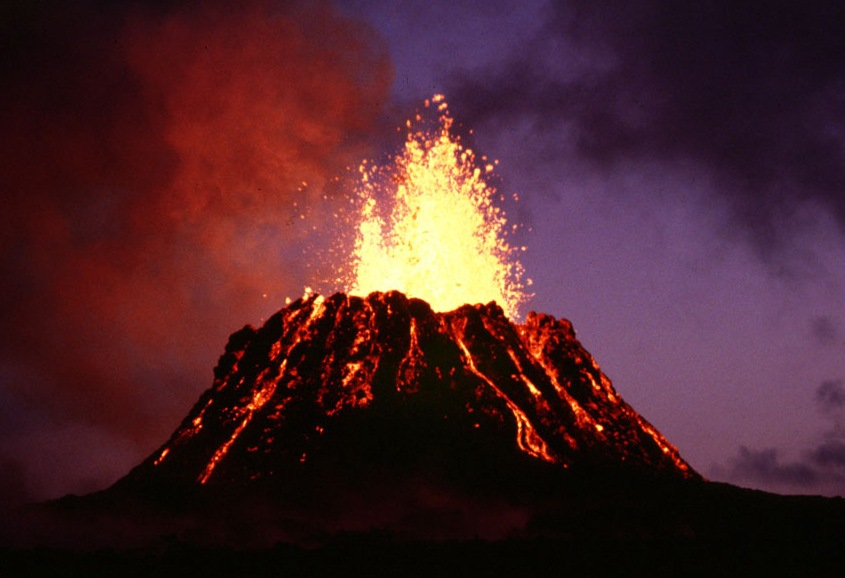
\includegraphics[width=0.55\linewidth]{images/book3/b1-puu-oo-1983.jpg}
\par\smallskip{\small Een lavafontein op de kegel Pu\textquoteleft
u~\textquoteleft O\textquoteleft o, op de oostelijke riftzone van de Kilauea,
29 juni 1983, in het eerste jaar van een uitbarsting die tientallen jaren duurde:
basaltlava, heet en dun, omhooggeslingerd in een straal en rond de krater
terugvallend. Foto: G.~E.~Ulrich, U.S. Geological Survey, publiek domein
(Wikimedia Commons).}
\label{fig:b1:hotspots:puu-oo}
\end{omfigure}
% ledger: commons:puu-oo, pp1801:kilauea-rate

\begin{history}[Een vast referentiekader voor de platen]
In 1963 verklaarde John Tuzo Wilson de Hawaïaanse eilanden, steeds ouder langs een lijn, door een bron van lava die in de trage kern van een mantelconvectiecel bleef, terwijl het snellere bovenste deel van de cel de zeebodem erover voerde. In 1971 en 1972 maakte W. Jason Morgan van die bron een pluim, ongeveer \qty{150}{km} breed, die uit het diepste deel van de \omterm{def:b1:layered-earth:layers}{mantel} opsteeg en daardoor bijna vast bleef terwijl de platen erboven bewogen; tankproeven toonden al snel hoe zo'n pluim eruitziet. De \omterm{def:b1:hotspots:hotspot}{hotspots} werden een kader waarin de platen tegen de \omterm{def:b1:layered-earth:layers}{mantel} konden worden gemeten, en niet alleen tegen elkaar. Een halve eeuw later blijkt het kader te bewegen, de Hawaïaanse \omterm{def:b1:hotspots:hotspot}{hotspot} onder meer, maar traag genoeg dat de Pacifische sporen de beweging van de plaat boven de \omterm{def:b1:layered-earth:layers}{mantel} nog steeds tot enkele graden en enkele centimeters per jaar geven, zoals de pasvorming in dit hoofdstuk liet zien.
\end{history}
% ledger: hist:plumes, tarduno:emperor

\section{Grote magmatische provincies}\label{sec:b1:hotspots:lips}

\begin{definition}[Grote magmatische provincie]\label{def:b1:hotspots:lip}
Een \emph{grote magmatische provincie}\index{grote magmatische provincie} (LIP) is een ophoping van stollingsgesteente, meestal basalt, die niet ontstaat door gewone spreiding bij een rug, meer dan \qty{e5}{km^2} bedekt, meer dan \qty{e5}{km^3} bevat en binnen hooguit ongeveer 50 miljoen jaar is geplaatst, het meeste ervan in pulsen van 1 tot 5 miljoen jaar die meer dan drie kwart van hun volume dragen. Op het land zijn LIP's meestal vloedbasalten; in de oceanen zijn het oceanische plateaus.
\end{definition}

Een typische LIP bedekt ongeveer een miljoen vierkante kilometer en bevat ongeveer een miljoen kubieke kilometer lava, het meeste ervan uitgestoten in ongeveer een miljoen jaar of minder. Hun lava's zijn opgestapeld in bijna vlakke stromen, die door erosie in treden worden gesneden: de \emph{trappen} waaraan zij hun naam danken. De tabel geeft de belangrijkste van de laatste 260 miljoen jaar.
% ledger: be08:definition, cr03:summary

\begin{omfigure}
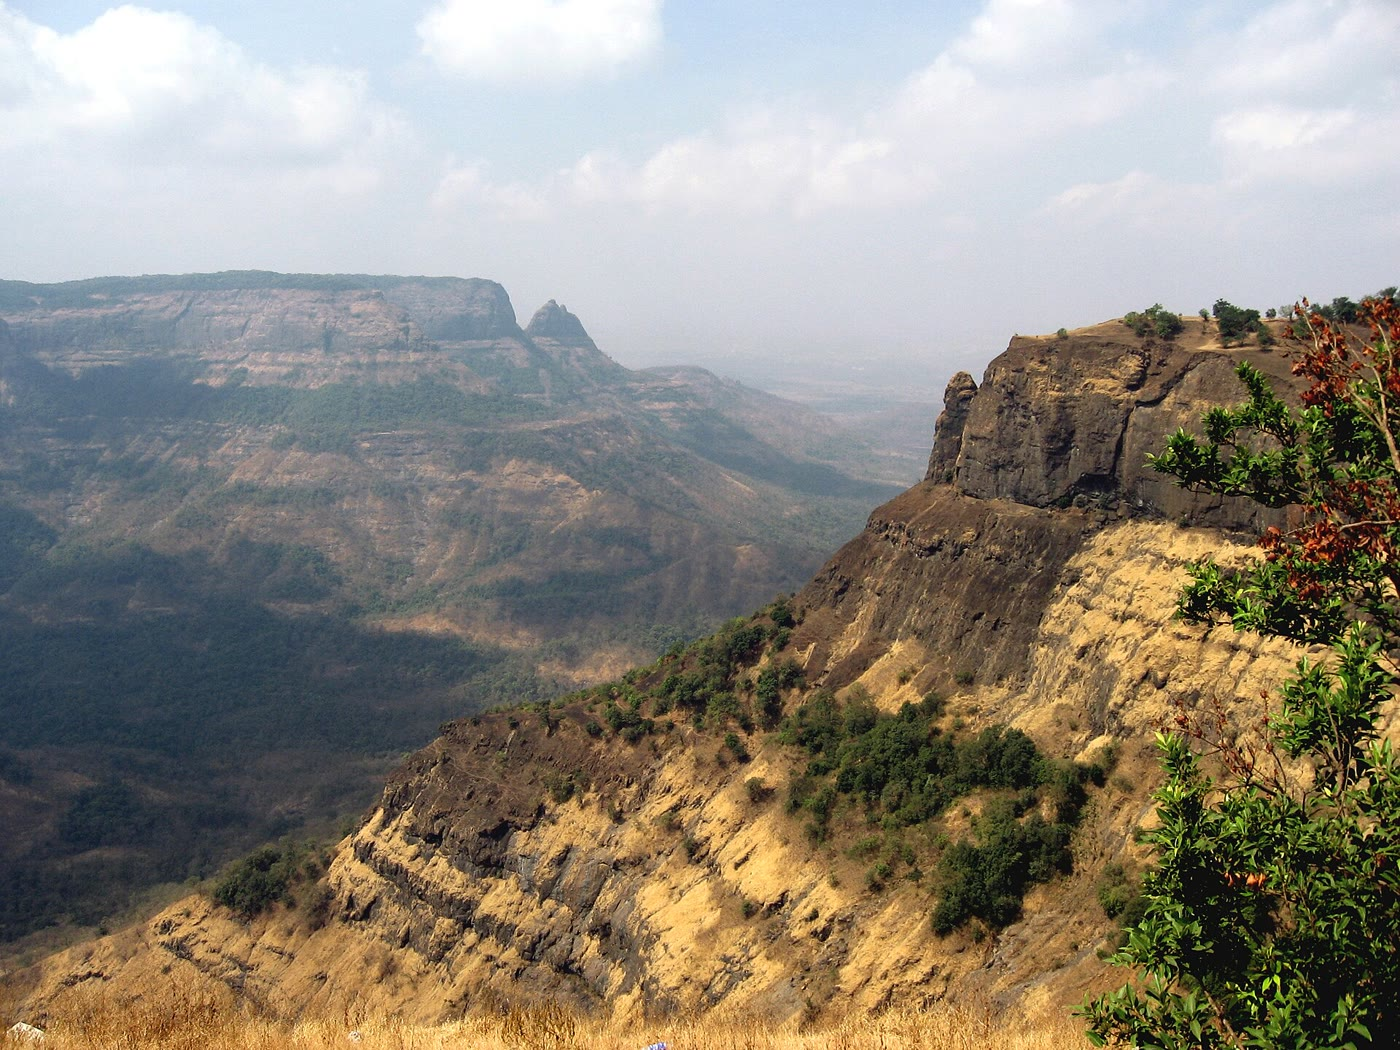
\includegraphics[width=0.55\linewidth]{images/book3/b1-deccan-matheran.jpg}
\par\smallskip{\small De Westelijke Ghats nabij Matheran, India: platte heuvels die in een stapel van bijna horizontale lavastromen van de Deccan-trappen zijn gesneden, waarvan de weerbestendige lagen de treden van de hellingen vormen. Foto: Nicholas (Nichalp), CC BY-SA 2.5 (Wikimedia Commons).}
\label{fig:b1:hotspots:deccan}
\end{omfigure}
% ledger: commons:matheran

\begin{center}
\small
\begin{tabular}{llll}
\hline
provincie & leeftijd (Ma) & oppervlakte (\unit{Mkm^2}) & eerste volume (\unit{Mkm^3})\\
\hline
Columbia River & 16 & 0.2 & 0.2\\
Ethiopië–Jemen & 30 & 0.7 & 1.2\\
Noord-Atlantische Oceaan & 61 en 56 & 1.2 & meer dan 2\\
Deccan & 65.5 & 0.5 (ooit 1.8) & 2 tot 4\\
Ontong Java & 122 en 90 & 2 & 44 (hele \omterm{def:b1:layered-earth:layers}{korst})\\
Paraná–Etendeka & 133 & 1.5 (ooit meer dan 2) & meer dan 2.3\\
Karoo–Ferrar & 183 & 3.1 & meer dan 2.5\\
Centrale Atlantische Oceaan (CAMP) & 201 & ooit tot 7 & meer dan 2\\
Siberische trappen & 250 & 0.4 (ooit meer dan 4) & meer dan 3\\
Emeishan & 259 & 0.5 (ooit 2 tot 5) & meer dan 1\\
\hline
\end{tabular}
\par\smallskip{\small Gemiddelde leeftijden; oppervlakten zoals zij nu zijn, en zoals zij bij de eerste uitbarsting waren waar een schatting bestaat; volumes van lava zoals bij de eerste uitbarsting, behalve voor het Ontong Java-plateau, waarvan het cijfer de hele verdikte \omterm{def:b1:layered-earth:layers}{korst} telt. Gegevens: V.~Courtillot en P.~Renne (2003).}
\end{center}
% ledger: cr03:table

\noindent Het pluimmodel dat in \cref{sec:b1:hotspots:plumes} is geschetst, verklaart zowel de omvang als de haast: een pluimkop van honderden kilometers breed bereikt de basis van de \omterm{def:b1:layered-earth:lithosphere}{lithosfeer}, ontspant en smelt, en overstroomt het oppervlak; daarna bouwt de staart gewoon een \omterm{def:b1:hotspots:track}{hotspotspoor} verder. Enkele provincies worden vermoed te staan aan het oude uiteinde van een nog levend spoor: de Deccan-trappen en de \omterm{def:b1:hotspots:hotspot}{hotspot} van Réunion, Paraná–Etendeka en Tristan da Cunha, verbonden door de Walvisrug, en de basalten van de Columbia River en Yellowstone.
% ledger: cr03:deccan (Reunion hot spot, plume-head model), be08:ojmh (Parana-Etendeka-Walvis-Tristan), pm90:track (Columbia River basalts)

De Deccan-trappen van midden-west India zijn een stapel lavastromen van ongeveer \qty{2500}{m} dik, waarvan minstens \qty{1800}{m} dicht bij 65.5 miljoen jaar geleden is uitgestoten, in veel minder dan een miljoen jaar; vandaag bedekken zij ongeveer \qty{0.5}{\mega km^2}, misschien \qty{1.8}{\mega km^2} vóór de erosie. Het Ontong Java-plateau, in de zuidwestelijke Stille Oceaan, is het grootste van alle oceanische plateaus: het bedekt ongeveer \qty{2}{\mega km^2}, en zijn \omterm{def:b1:layered-earth:layers}{korst}, ongeveer \qty{36}{km} dik, bevat ongeveer \qty{44}{\mega km^3} stollingsgesteente. De plateaus van Manihiki en Hikurangi, nu ver ervandaan over jongere oceaanbodem, kunnen samen met het Ontong Java-plateau één plateau hebben gevormd. De Centrale Atlantische Magmatische Provincie, ongeveer 201 miljoen jaar geleden uitgestoten toen de Atlantische Oceaan begon te openen, ligt vandaag verspreid, als lava's, dijken en sills, over vier continenten: het oosten van Noord-Amerika, het noordoosten van Zuid-Amerika, West-Afrika en het zuidwesten van Europa; zij heeft misschien eens tot \qty{7}{\mega km^2} bedekt.
% ledger: cr03:deccan, cr03:table, cr03:ontong-java, be08:ojmh, cr03:camp


Enkele provincies vallen in de tijd samen met de grote massa-extincties die de biologie beschrijft: de Siberische trappen met de grootste van alle, aan het einde van het Perm; de Centrale Atlantische provincie met het einde van het Trias; de Karoo–Ferrar met een uitsterving in het vroege Jura; de Emeishan met een in het midden-Perm; en de Deccan-trappen met het einde van het Krijt. De vier grootste extincties van de laatste 260 miljoen jaar vallen elk, voor zover de dateringen dat kunnen zeggen, samen met een van deze provincies, en een oorzakelijk verband wordt het meest waarschijnlijk geacht. De voorgestelde mechanismen zijn atmosferisch: sulfaataerosolen die het klimaat voor korte tijd afkoelen, koolstofdioxide dat het veel langer verwarmt, en oceanen die zonder zuurstof komen te zitten. Voor het einde van het Krijt begonnen de Deccan-uitbarstingen vóór de inslag bij Chicxulub en gingen zij erna door; een overzicht van de gegevens over de grens concludeerde in 2010 dat de inslag de uitsterving heeft veroorzaakt.
% ledger: cr03:table, cr03:summary, cr03:deccan, schulte:kpg

Niet al het vulkanisme ver van de plaatgrenzen heeft een pluim nodig. Kleine vulkanische velden groeien waar een plaat wordt uitgerekt of gebarsten, en de ketens zonder een zuivere leeftijdsprogressie worden misschien gevoed vanuit de bovenste \omterm{def:b1:layered-earth:layers}{mantel}; dit is de platenhypothese aan het werk. Wat de oceanische eilanden worden nadat de \omterm{def:b1:hotspots:hotspot}{hotspot} hen heeft verlaten, terwijl zij wegzakken, verweren en riffen laten groeien, hoort bij Boek 4.
% ledger: fn03:plate-hypothesis

\section{Oefeningen}

\begin{exercise}[$\star$]\label{exo:b1:hotspots:1}
(a) Mauna Kea steekt \qty{4205}{m} boven zeeniveau uit, en de zeebodem ver van de Hawaïaanse keten ligt \qty{5274}{m} diep. Bereken hoe hoog de vulkaan boven die bodem staat. Leg uit waarom haar ware hoogte vanaf haar voet nog groter is. (b) Mauna Loa bevat ongeveer \qty{74000}{km^3}. Bereken hoe lang het zou duren om haar op te bouwen met de huidige aanvoer van de Kilauea, \qty{0.1}{km^3} per jaar, en met de gemiddelde aanvoer van de hele keten, \qty{0.025}{km^3} per jaar. (c) De Pu\textquoteleft
u~\textquoteleft O\textquoteleft o-uitbarsting stroomde van 1983 tot 2002 ongeveer \qty{0.12}{km^3} per jaar uit. Bereken welk volume dat is, en welk deel van Mauna Loa het is.
% ledger: pp1801:volumes, pp1801:kilauea-supply, pp1801:chain-volume, pp1801:kilauea-rate; 5274 m from hotspots.py
\end{exercise}

\begin{exercise}[$\star$]\label{exo:b1:hotspots:2}
Een plaat draait over de \omterm{def:b1:hotspots:hotspot}{hotspots} met \qty{0.92}{\degree\per\Myr}. Neem $R = \qty{6371}{km}$. (a) Druk $\omega$ uit in radialen per miljoen jaar. (b) Bereken de snelheid, in \unit{mm.yr^{-1}}, van de \omterm{def:b1:hotspots:hotspot}{hotspots} op \ang{30}, \ang{60}, \ang{90} en \ang{108.0} van de pool. (c) Leg uit waarom de snelheid van Hawaï, op \ang{108.0}, kleiner is dan op \ang{90}.
\end{exercise}

\begin{exercise}[$\star$]\label{exo:b1:hotspots:3}
(a) Bereken de gemiddelde dikte van de Deccan-trappen zoals zij nu zijn, \qty{1}{\mega km^3} over \qty{0.5}{\mega km^2}, en van de Centrale Atlantische provincie, \qty{2}{\mega km^3} over \qty{7}{\mega km^2}. (b) Vergelijk met de dikte van de Deccan-doorsnede, \qty{2500}{m}. (c) Leg uit waarom de gemiddelde dikte van de Centrale Atlantische provincie weinig zegt over de dikte van haar lavapakketten.
% ledger: cr03:table, cr03:deccan, cr03:camp
\end{exercise}

\begin{exercise}[$\star$]\label{exo:b1:hotspots:4}
Pluimgesteente dat \qty{250}{K} heter is dan de \omterm{def:b1:layered-earth:layers}{mantel} eromheen heeft $\alpha = \qty{3.2e-5}{K^{-1}}$ en $\rho_m = \qty{3300}{kg.m^{-3}}$. (a) Bereken hoeveel het lichter is, in \unit{kg.m^{-3}}. (b) Bereken welke dikte van zulk gesteente, uitgespreid onder de plaat, een opwelling van \qty{690}{m} hoog onder de zee isostatisch zou ondersteunen ($\rho_w = \qty{1000}{kg.m^{-3}}$)?
% ledger: herzberg:tp (200-300 K), parsons:plate-model (alpha)
\end{exercise}

\begin{exercise}[$\star\star$]\label{exo:b1:hotspots:5}
Twee \omterm{def:b1:hotspots:hotspot}{hotspots} liggen op de evenaar, A op \ang{0}\,E en B op \ang{90}\,E, en beide sporen lopen recht naar het westen (\omterm{def:b1:spherical-astronomy:horizontal}{azimut} \ang{270}). (a) Bereken de spoorvectoren $\vec t_A$ en $\vec t_B$. (b) Bereken $\vec t_A\times\vec t_B$. (c) Pas de tekenregel van \cref{prop:b1:hotspots:two-tracks} toe en bepaal waar de \omterm{def:b1:plate-kinematics:euler-pole}{Eulerpool} ligt; verklaar het resultaat zonder berekening. (d) Als A met \qty{50}{mm.yr^{-1}} beweegt, bereken $\omega$ in graden per miljoen jaar.
\end{exercise}

\begin{exercise}[$\star\star$]\label{exo:b1:hotspots:6}
Drie \omterm{def:b1:hotspots:hotspot}{hotspots} van één plaat liggen op de afstanden $x = R\sin\Delta = 3000$, 5000
en \qty{6000}{km} van de rotatieas en bewegen met 30, 48 en
\qty{57}{mm.yr^{-1}}. (a) Pas $v = \omega x$ aan met de kleinste kwadraten en geef
$\omega$ in radialen en in graden per miljoen jaar. (b) Bereken de
residuen. (c) Leg uit waarom de lijn door de oorsprong moet gaan.
\end{exercise}

\begin{exercise}[$\star\star$]\label{exo:b1:hotspots:7}
Een opwelling met doorsnede \qty{3e8}{m^2} omringt een \omterm{def:b1:hotspots:track}{hotspotspoor} op een plaat die met
\qty{50}{mm.yr^{-1}} beweegt. Neem $\rho_m - \rho_w = \qty{2300}{kg.m^{-3}}$,
$c_p = \qty{910}{J.kg^{-1}.K^{-1}}$ en $\alpha = \qty{3.2e-5}{K^{-1}}$. (a)
Bereken de opdrijvingsflux en de \omterm{def:b1:heat-budget:heat-flow}{warmtestroom}. (b) Vergelijk met Hawaï,
\qty{3240}{kg.s^{-1}}. (c) Twee \omterm{def:b1:hotspots:hotspot}{hotspots} hebben dezelfde opwelling; één ligt onder een plaat die twee keer zo snel beweegt. Bepaal welke pluim sterker is.
\end{exercise}

\begin{exercise}[$\star\star$]\label{exo:b1:hotspots:8}
Langs het Yellowstone-spoor begonnen de caldera-uitbarstingen in het McDermitt-vulkaanveld 16.1 miljoen jaar geleden, en in het Picabo-veld, ongeveer \qty{350}{km} naar het noordoosten, 10.3 miljoen jaar geleden; sindsdien zijn zij met $\qty[uncertainty-mode=separate]{2.9 \pm 0.5}{cm}$ per jaar naar N\,\ang{54}\,E verschoven. (a) Bereken de gemiddelde snelheid waarmee het vulkanisme van McDermitt naar Picabo is gemigreerd. (b) Vergelijk beide snelheden met die van de plaat boven de \omterm{def:b1:hotspots:hotspot}{hotspot}, \qty[uncertainty-mode=separate]{26 \pm 5}{mm.yr^{-1}} naar \ang{235}. (c) Controleer of de richting van het jonge spoor de verwachte is. (d) Het oudere deel van het spoor ligt in een gebied dat is uitgerekt terwijl het vulkanisme passeerde. Leg uit hoe dat het verschil kan verklaren.
% ledger: pm90:track, data:b3-hotspots
\end{exercise}

\begin{exercise}[$\star\star$]\label{exo:b1:hotspots:9}
De Hawaïaanse pluim draagt ongeveer \qty{9.2e10}{W} aan overtollige warmte. (a) Bereken, als die geheel door de \qty{1000}{km} bij \qty{1000}{km} zeebodem het dichtst bij de \omterm{def:b1:hotspots:hotspot}{hotspot} zou verlaten, met hoeveel de \omterm{def:b1:heat-budget:heat-flow}{warmtestroom} daar zou stijgen. (b) Vergelijk met de waargenomen overtollige warmte, hoogstens 5 tot \qty{10}{mW.m^{-2}}. (c) Bereken hoe lang warmte nodig heeft om door een plaat van \qty{100}{km} dik te diffunderen ($\kappa = \qty{e-6}{m^2.s^{-1}}$), en hoe lang de plaat erover doet om \qty{1000}{km} af te leggen met \qty{92}{mm.yr^{-1}}. Trek een conclusie.
% ledger: vh89:swell-heat
\end{exercise}

\begin{exercise}[$\star\star\star$]\label{exo:b1:hotspots:10}
De Deccan-trappen bevatten ongeveer \qty{e6}{km^3} lava. Neem aan dat zij afkomstig is van een bolvormig pluimhoofd waarvan een tiende is gesmolten. (a) Bereken het volume en de straal van het hoofd. (b) Bereken welke diameter het hoofd zou hebben als het tot een schijf van \qty{100}{km} dik was platgedrukt onder de \omterm{def:b1:layered-earth:lithosphere}{lithosfeer}. Vergelijk het oppervlak ervan met het oppervlak dat de trappen misschien eens hebben bedekt, \qty{1.8}{\mega km^2}. (c) Vergelijk, als de lava in één miljoen jaar is uitgestoten, de snelheid ervan met de huidige aanvoer van de Kilauea, \qty{0.1}{km^3} per jaar. (d) Leg uit waarom een pluimhoofd groot moet zijn, terwijl de staart die volgt smal is.
% ledger: cr03:table, pp1801:kilauea-supply
\end{exercise}

\begin{exercise}[$\star\star\star$]\label{exo:b1:hotspots:11}
Tussen 81 en 47 miljoen jaar geleden bewoog de Hawaïaanse \omterm{def:b1:hotspots:hotspot}{hotspot} naar het zuiden met meer dan \qty{40}{mm.yr^{-1}}. (a) Neem \qty{40}{mm.yr^{-1}} aan en bereken hoe ver hij is verschoven.
(b) Neem aan dat de plaat zich in die tijd met \qty{80}{mm.yr^{-1}} naar \ang{340} bewoog over de diepe \omterm{def:b1:layered-earth:layers}{mantel}. Bereken, met $x$ naar het oosten en $y$ naar het noorden, de snelheid van de plaat ten opzichte van de wegdrijvende \omterm{def:b1:hotspots:hotspot}{hotspot}, haar snelheid en haar \omterm{def:b1:spherical-astronomy:horizontal}{azimut}. (c) Bereken met hoeveel procent, en met hoeveel graden, een spoor dat toen werd gevormd de beweging van de plaat over de diepe \omterm{def:b1:layered-earth:layers}{mantel} verkeerd zou weergeven.
% ledger: tarduno:emperor
\end{exercise}

\begin{exercise}[$\star\star\star$]\label{exo:b1:hotspots:12}
(a) Een vloedbasalt van \qty{e6}{km^3} koelt af van ongeveer \qty{1300}{\celsius} tot de temperatuur van het oppervlak. Neem een warmtecapaciteit van \qty{3}{MJ.m^{-3}.K^{-1}} en bereken hoeveel warmte zij afgeeft (negeer de latente warmte van kristallisatie). (b) Bereken, over één miljoen jaar uitgespreid, welk vermogen dat is. Vergelijk dat met dat van de Hawaïaanse pluim, \qty{9.2e10}{W}, en met de \qty{47}{TW} van de hele Aarde. (c) Een pluimhoofd verwarmt ook de basis van de \omterm{def:b1:layered-earth:lithosphere}{lithosfeer} zonder haar geheel te doen smelten. Ga na of het vermogen van (b) een bovengrens of een ondergrens is voor de warmte die het hoofd aanvoert.
% ledger: delaney86:properties (Book 2 row, 2-3 MJ/m3/K), dd10:total; 1300 degC is an exercise value
\end{exercise}

\section{Probleem: de snelheidsmeter van de Pacifische plaat}

\begin{problem}[{Weekendprobleem --- de Eulerpool van de Pacifische plaat uit twee hotspotsporen, haar snelheid uit een derde meting, een toets aan andere hotspots, en de opdrijving en aanvoer van de Hawaïaanse pluim}]
\label{pb:b1:hotspots:1}
% values: calc/ch15.py; ledger: data:b3-hotspots, data:etopo1, pp1801:kilauea-supply, pp1801:volumes,
% pp1801:chain-volume, delaney86:properties, parsons:plate-model, dd10:total, data:pb2002 (ridge_budget.py), cd87:rate
Morgan en Morgan geven de Hawaïaanse \omterm{def:b1:hotspots:hotspot}{hotspot} op \ang{19.0}\,N, \ang{155.2}\,W, met een spoor naar $\ang{304}\pm\ang{3}$ en een snelheid van \qty[uncertainty-mode=separate]{92 \pm 3}{mm.yr^{-1}}, en de \omterm{def:b1:hotspots:hotspot}{Louisville-hotspot} op \ang{53.6}\,S, \ang{140.6}\,W, met een spoor naar $\ang{316}\pm\ang{5}$ en een snelheid van \qty[uncertainty-mode=separate]{67 \pm 5}{mm.yr^{-1}}. Gebruik de assen en de vectoren $\vec e$, $\vec n$, $\vec t$ van \cref{sec:b1:hotspots:tracks}, met $R = \qty{6371}{km}$. Geef de componenten tot vier decimalen.

\medskip
\noindent\textbf{Deel I --- De pool uit twee sporen.}
\begin{enumerate}
  \item Bereken $\vec r$, $\vec e$ en $\vec n$ in Hawaï, en daarna de spoorvector
        $\vec t_H$.
  \item Doe hetzelfde bij Louisville: $\vec r_L$, $\vec e$, $\vec n$ en
        $\vec t_L$.
  \item Controleer dat $\vec t_H$ een eenheidsvector is die loodrecht staat op $\vec r_H$.
  \item Bereken $\vec t_H\times\vec t_L$ en de lengte ervan. Bepaal de hoek die de twee
        spoorvectoren maken.
  \item Normeer het kruisproduct en pas de tekenregel toe van
        \cref{prop:b1:hotspots:two-tracks}.
  \item Geef de breedte- en \omterm{def:b1:spherical-astronomy:geographic}{lengtegraad} van de \omterm{def:b1:plate-kinematics:euler-pole}{Eulerpool} van de Pacifische plaat
        ten opzichte van de \omterm{def:b1:hotspots:hotspot}{hotspots}.
\end{enumerate}

\medskip
\noindent\textbf{Deel II --- De snelheid.}
\begin{enumerate}[resume]
  \item Bereken de hoekafstanden $\Delta_H$ en $\Delta_L$ van de pool
        tot de twee \omterm{def:b1:hotspots:hotspot}{hotspots}.
  \item Bereken $(\vec p\times\vec r_L)\cdot\vec t_L$. Leg uit waarom het gelijk is aan
        $\sin\Delta_L$, en wat het teken ervan zegt over de beweging bij Louisville.
  \item Bereken uit de snelheid bij Louisville $\omega$ in radialen en in
        graden per miljoen jaar.
  \item Bereken hoe lang de Pacifische plaat erover doet om één volledige
        omwenteling om deze pool te maken.
  \item De kleinste-kwadratenpool van de vijftien Pacifische sporen ligt op
        \ang{63.78}\,S, \ang{112.48}\,E, met \qty{0.92}{\degree\per\Myr}.
        Bereken de hoek tussen de twee polen en vergelijk de twee snelheden.
\end{enumerate}

\medskip
\noindent\textbf{Deel III --- Een toets aan drie andere hotspots.} Morgan en
Morgan geven de \omterm{def:b1:hotspots:hotspot}{Society-hotspot} (\ang{18.2}\,S, \ang{148.4}\,W)
\qty[uncertainty-mode=separate]{109 \pm 10}{mm.yr^{-1}}, Pitcairn
(\ang{25.4}\,S, \ang{129.3}\,W)
\qty[uncertainty-mode=separate]{90 \pm 15}{mm.yr^{-1}} en Cobb
(\ang{46.0}\,N, \ang{130.1}\,W)
\qty[uncertainty-mode=separate]{43 \pm 3}{mm.yr^{-1}}.
\begin{enumerate}[resume]
  \item Bereken de hoekafstand van de pool uit vraag 6 tot elk van de
        drie \omterm{def:b1:hotspots:hotspot}{hotspots}.
  \item Voorspel de drie snelheden met de snelheid uit vraag 9.
  \item Ga na welke voorspellingen overeenstemmen met de gemeten snelheden binnen
        hun onzekerheden, en welke niet.
  \item Twee sporen met verschillende richtingen geven altijd een pool. Leg uit waarom
        twee bijna evenwijdige sporen een slechte keuze zijn.
\end{enumerate}

\medskip
\noindent\textbf{Deel IV --- De pluim en de snelheidsmeter.} De Hawaïaanse opwelling
heeft de doorsnede \qty{4.83e8}{m^2}. Neem
$\rho_m - \rho_w = \qty{2300}{kg.m^{-3}}$, $c_p = \qty{910}{J.kg^{-1}.K^{-1}}$
en $\alpha = \qty{3.2e-5}{K^{-1}}$.
\begin{enumerate}[resume]
  \item Reken \qty{92}{mm.yr^{-1}} om naar \unit{m.s^{-1}} en bereken de
        opdrijvingsflux van de Hawaïaanse pluim.
  \item Bereken de overtollige warmte die zij draagt, en vergelijk met de
        \qty{47}{TW} die de Aarde verlaten.
  \item De ruggen maken ongeveer \qty{21}{km^3} \omterm{def:b1:layered-earth:layers}{korst} per jaar langs ongeveer
        \qty{67000}{km}. Bereken welke lengte van rug evenveel \omterm{def:b1:layered-earth:layers}{korst} maakt als de
        Kilauea er per jaar van krijgt, \qty{0.1}{km^3}.
  \item Bereken met dat tempo hoe lang Mauna Loa, ongeveer \qty{74000}{km^3},
        nodig heeft om te groeien.
  \item De \omterm{def:b1:hotspots:hotspot}{hotspot} bouwde in 81 miljoen jaar ongeveer \qty{2e6}{km^3} van de keten
        op. Bereken haar gemiddelde productie en vergelijk die met de huidige aanvoer van de Kilauea.
  \item Bereken, met de pool en de snelheid uit delen I en II, de snelheid die het
        Louisville-spoor voor de Pacifische plaat boven de Hawaïaanse \omterm{def:b1:hotspots:hotspot}{hotspot} voorspelt.
  \item Vergelijk met de gemeten \qty[uncertainty-mode=separate]{92 \pm 3}{mm.yr^{-1}}: bereken met hoeveel ze verschillen, en met hoeveel standaardonzekerheden.
  \item Uit de leeftijden van de Hawaïaanse vulkanen vond Boek 2 \qty{9.1}{cm} per
        jaar, en de auteurs van de leeftijden, die de hele keten pasten, vonden
        \qty{8.6}{cm} per jaar. Vergelijk deze gemiddelden over tientallen miljoenen
        jaar met de twee snelheden van de \omterm{def:b1:hotspots:hotspot}{hotspots}.
  \item Geef tot één decimaal, in centimeter per jaar, welke snelheid het
        Louisville-spoor de Pacifische plaat boven de Hawaïaanse \omterm{def:b1:hotspots:hotspot}{hotspot} geeft.
\end{enumerate}
\end{problem}
